\documentclass[compress]{beamer}

\usetheme{Hamburg}

\usepackage[T1]{fontenc}
\usepackage[utf8]{inputenc}

\usepackage{lmodern}

%\usepackage[english]{babel}
\usepackage[ngerman]{babel}

\usepackage{eurosym}
\usepackage{listings}
\usepackage{microtype}
\usepackage{units}
\usepackage{hyperref}
\usepackage{url}


\lstset{
	basicstyle=\ttfamily\footnotesize,
	frame=single,
	numbers=left,
	language=C,
	breaklines=true,
	breakatwhitespace=true,
	postbreak=\hbox{$\hookrightarrow$ },
	showstringspaces=false,
	tabsize=4,
	captionpos=b,
	morekeywords={gboolean,gpointer,gconstpointer,gchar,guchar,gint,guint,gshort,gushort,glong,gulong,gint8,guint8,gint16,guint16,gint32,guint32,gint64,guint64,gfloat,gdouble,gsize,gssize,goffset,gintptr,guintptr,int8_t,uint8_t,int16_t,uint16_t,int32_t,uint32_t,int64_t,uint64_t,size_t,ssize_t,off_t,intptr_t,uintptr_t,mode_t}
}

\title{I/O analysis of climate applications}
\author{Arne Beer \& Frank Röder}
\institute{Arbeitsbereich Wissenschaftliches Rechnen\\Fachbereich Informatik\\Fakultät für Mathematik, Informatik und Naturwissenschaften\\Universität Hamburg}
\date{2016-07-2}

\titlegraphic{
\includegraphics[width=0.75\textwidth]{gfx/logo}}

\begin{document}

\begin{frame}
	\titlepage
\end{frame}

\begin{frame}
	\frametitle{Content (Agenda)}

	\tableofcontents[hidesubsections]
\end{frame}

\section{Introduction}
\subsection{Subsection}

%\section{Models}
%\begin{frame}
%    \frametitle{Models}
%
%    \begin{itemize}
%        \item
%    \end{itemize}
%
%\end{frame}


\begin{frame}
	\frametitle{Introduction}

	\begin{itemize}
		\item Climate Applications
		\begin{itemize}
			\item About the I/O
			\item Analysis
			\item different Models
			\item Visualisation
		\end{itemize}
	\end{itemize}

\end{frame}


\section{Models}
\begin{frame}
    \frametitle{What are models}

    \begin{itemize}
		\item Climate Models
		\begin{itemize}
			\item A representation for climate
			\item Ocean, Ice, Land, River, Vegetation
			\item Predict future climate
			\item Global scale
		\end{itemize}

		\item Atmospherical model
		\begin{itemize}
			\item Numerical Weather Prediction
			\item Predict weather in a forseeable period
		\end{itemize}
    \end{itemize}

\end{frame}


\section{Input and Output}
\subsection{Data}

\begin{frame}[fragile]
	\frametitle{Structure of the data}

		\begin{itemize}
		    \item Numeric data
			\item Scalar quantities
			\item Vectors
			\item grit data
		\end{itemize}

\end{frame}

\subsection{File Format}

\begin{frame}[fragile]
	\frametitle{Most important formats used for climate applications}

		\begin{itemize}
			\item netCDF
			\item HDF5
			\item Since version 4 netCDF is embedded in HDF5
		\end{itemize}

  \begin{figure}[htbp]
    \begin{minipage}{0.35\textwidth}
     \centering
      
\includegraphics[width=0.8\textwidth]{gfx/hdf.jpg}
      \caption{hdf-logo \cite{hdf}}
    \end{minipage}\hfill
    \begin{minipage}{0.35\textwidth}
     \centering
      
\includegraphics[width=0.8\textwidth]{gfx/netcdf.png}
      \caption{netcdf-logo \cite{netcdf}}
    \end{minipage}
  \end{figure}

\end{frame}


\section{The model landscape}
\begin{frame}
    \frametitle{The model landscape}

		\begin{itemize}
		    \item Large choice
			\item Old models
			\item Poorly documented
			\item Nearly no open source
		\end{itemize}

\end{frame}

\section{Awips II}
\begin{frame}
    \frametitle{Awips II}
    \begin{center}
    	\begin{figure}
			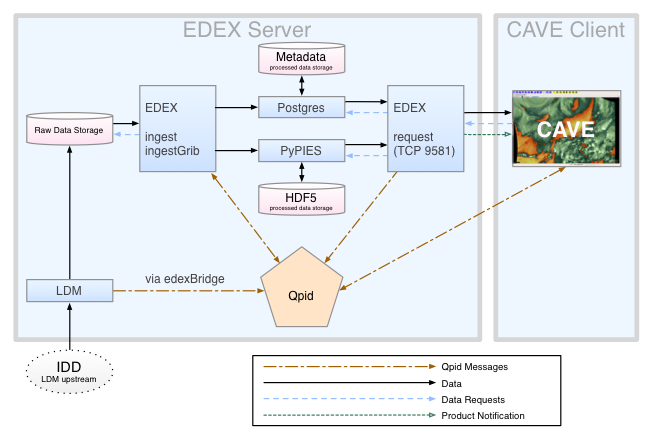
\includegraphics[width=0.7\textwidth]{gfx/awipsII.png}
      	  	\caption[]{Awips Infrastructure \cite{Uni01}}
		\end{figure}
	\end{center}

\end{frame}

\begin{frame}
    \frametitle{Awips II}
    	\begin{itemize}
			\item Forecast display and analysis
			\item Provides EDEX to store computed data
	    	\begin{itemize}
		    	\item HDF5 Storage
		    	\item Custom Python libraries for storage management
		    	\item PostgreSQL for metadata management and storage
		    \end{itemize}
		    \item Provides CAVE to display data
	    	\begin{itemize}
		    	\item Program to connect with EDEX server
		    	\item Select data set, download and view it on your local machine
		    \end{itemize}
		\end{itemize}
\end{frame}


\begin{frame}
    \frametitle{CESM}
    	\begin{itemize}
    	    \item Community Earth System Model
			\item Model for global climate simulation
			\item Provides scripts for setting up the machine in 4 commands
	    	\begin{itemize}
		    	\item Scripts are broken
		    	\item Mix of bash, csh, perl
		    \end{itemize}
		    \item Good configurability with xml files.
		\end{itemize}
\end{frame}


\section{Zusammenfassung}
\subsection*{}

\begin{frame}
	\frametitle{Zusammenfassung}

	\begin{itemize}
		\item Data

		\begin{itemize}
			\item hdf5 , netCDF
		\end{itemize}

		\item Models
		\begin{itemize}
			\item awips2
			\item CESM
		\end{itemize}

		\item Quelle: \cite{Quelle2012}

	\end{itemize}
\end{frame}

\section{Literatur}
\subsection*{}

\begin{frame}
	\frametitle{Literatur}
    \frametitle{Quellenverzeichnis}

	\bibliographystyle{alpha}
	\bibliography{literatur.bib}
\end{frame}


\end{document}
